\documentclass[12pt]{article}

\usepackage{sbc-template}
\usepackage{graphicx}
\usepackage{url}
\usepackage[utf8]{inputenc}
\usepackage[T1]{fontenc}
\usepackage[brazilian]{babel}
\usepackage{array}

\sloppy

\title{Spatiotemporal Prediction of Robbery Occurrences \\ in the City of São Paulo Using Machine Learning \\ and Public Data}

\author{Luciana P. Nedel\inst{1}, Wesley Fernandes\inst{2}\\ Diego Soares de Carvalho Junior\inst{1}, Eduardo Nunes Martins\inst{3}}

\address{Escola de Artes, Ciências e Humanidades -- Universidade de São Paulo
  (USP)\\
  Address: Rua Arlindo Béttio, 1000 - Ermelino Matarazzo, São Paulo - SP, 03828-000
  \email{wesley.fernan1@usp.br, nome@usp.br, nome@usp.br}
}

\begin{document}
\maketitle

\section{Resumo}

O objetivo geral deste trabalho é desenvolver e comparar modelos de aprendizado de máquina para prever a incidência de roubos na cidade de São Paulo a partir de padrões históricos, espaciais e temporais presentes em dados públicos de segurança e socioeconômicos. A incidência será representada pela contagem de registros de roubo por área e período; inicialmente, considera-se o par bairro--dia. Nesta etapa, foram examinados dados da Secretaria da Segurança Pública do Estado de São Paulo (SSP-SP) referentes a registros de 2022 a 2026. A análise exploratória distinguiu a data da ocorrência da data de registro e descreveu padrões temporais, espaciais e problemas de qualidade dos dados. Para ocorrências em 2025, foram identificados 107.750 registros nos arquivos disponíveis, com média aproximada de 295 por dia. No arquivo de registros de 2025, 11,5\% dos roubos atribuídos à capital não têm coordenadas utilizáveis. A integração de indicadores socioeconômicos e a comparação preditiva ainda não foram realizadas.

\section{Introdução}

Os registros de roubo em uma cidade grande variam no espaço e no tempo. Entender essa variação é necessário antes de construir modelos que estimem quantos registros poderão ocorrer em uma região e em um período futuro. Na cidade de São Paulo, a SSP-SP disponibiliza microdados que incluem a data, o bairro e, em parte dos casos, as coordenadas da ocorrência \cite{ssp}. Esses campos permitem investigar padrões históricos, mas também trazem desafios: o local pode estar ausente, um mesmo bairro pode ser registrado com grafias diferentes e a data do registro pode ser posterior à data do fato.

A pergunta deste projeto é: em que medida padrões históricos, espaciais e temporais dos dados de segurança, combinados a indicadores socioeconômicos, permitem prever a quantidade de registros de roubo por área e período futuro na cidade de São Paulo? A unidade inicial de análise é o par bairro--dia, sujeita à avaliação da qualidade dos dados. Assim, o mapa de calor planejado representará contagens previstas para períodos futuros, após a construção e avaliação dos modelos. Mapas e gráficos desta entrega descrevem apenas registros observados.

O objetivo geral da pesquisa é desenvolver e comparar modelos de aprendizado de máquina para prever a incidência de roubos na cidade de São Paulo a partir de padrões históricos, espaciais e temporais presentes em dados públicos de segurança e socioeconômicos. Para tornar esse objetivo verificável, a incidência será operacionalizada como a contagem de registros de roubo por área e período, e os modelos serão comparados por seus erros em períodos posteriores aos usados no treinamento. Random Forest e XGBoost são os modelos inicialmente selecionados. Nesta entrega, o recorte é definido, a qualidade dos campos necessários é verificada e os padrões temporais e espaciais são descritos. Indicadores do Censo 2022 do IBGE estão previstos para a etapa de modelagem, após a compatibilização das unidades geográficas \cite{ibge}; essa integração ainda não foi realizada.

\section{Trabalhos Relacionados}

Ribeiro et al. \cite{ribeiro2022} estudaram a previsão de ocorrência de homicídio no mês seguinte em Belém, no Pará. O estudo combinou registros de 34 tipos de crime com informações de tempo e espaço e comparou métodos de classificação. Random Forest alcançou 76\% de acerto nas duas classes relatadas pelos autores. O resultado motiva a avaliação de modelos baseados em árvores, mas sua tarefa de classificação de homicídios difere da previsão de contagens diárias de roubos proposta aqui.

García-Zanabria et al. \cite{crimanalyzer} apresentaram o \textit{CrimAnalyzer}, sistema de análise visual de padrões criminais em São Paulo. O trabalho explora a variação espacial e temporal dos registros e a identificação de áreas com padrões relevantes para especialistas. Sua contribuição é especialmente próxima da análise exploratória e da visualização planejadas neste projeto. O sistema, contudo, não fornece uma comparação direta entre os modelos de regressão aqui propostos.

Hassan et al. \cite{hassan2024} investigaram a previsão de crimes na cidade de São Paulo por meio de redes neurais em grafos, integrando registros criminais, rede viária e dados urbanos. A pesquisa mostra uma forma de representar relações espaciais mais complexas. Este projeto começa com modelos para dados tabulares e uma unidade bairro--dia, o que permite avaliar primeiro a utilidade dos padrões históricos e temporais antes de considerar representações espaciais mais elaboradas.

\section{Método}

\subsection{Fonte, recorte e tratamento}

Foram utilizadas cinco planilhas anuais da SSP-SP, de 2022 a 2026 \cite{ssp}. O arquivo de 2026 disponível nesta análise contém o primeiro semestre. Cada registro foi selecionado quando o campo \texttt{NATUREZA\_APURADA} começava por ``ROUBO'' e o município da circunscrição do local do fato era São Paulo. Esse filtro inclui as categorias ``roubo -- outros'', ``roubo de veículo'', ``roubo de carga'' e ``roubo a banco''. O campo \texttt{NOME\_MUNICIPIO} ou \texttt{CIDADE} foi preservado apenas para conferência, pois o dicionário da base o descreve como município do registro, que pode diferir do local do fato.

Para a série temporal, foi utilizada \texttt{DATA\_OCORRENCIA\_BO}, e não o ano do arquivo. Registros de fatos ocorridos em um ano podem aparecer em arquivos posteriores. As planilhas também mudaram a posição de algumas colunas ao longo dos anos; por isso, os campos foram identificados pelo nome em cada arquivo. Na análise espacial, os nomes de bairro foram usados como aparecem na fonte, sem inferir equivalência entre grafias. Coordenadas ausentes ou iguais a zero não foram usadas para localizar pontos em mapas.

\subsection{Unidade de previsão e avaliação planejada}

A unidade inicialmente proposta para a previsão é bairro--dia, com a contagem de registros de roubo como variável resposta. Antes do treinamento, será necessário padronizar os nomes de bairro e formar pares bairro--dia também para dias sem registros. A distribuição dessas contagens indicará se a unidade diária deve ser mantida ou agregada em períodos mais longos.

Os candidatos iniciais são Random Forest e XGBoost aplicados à regressão. Variáveis temporais conhecidas antecipadamente, como dia da semana e mês, poderão ser combinadas com contagens históricas defasadas, informações espaciais e indicadores socioeconômicos do Censo 2022 após sua compatibilização geográfica. Nenhuma variável do período futuro, como hora ou local de um crime ainda desconhecido, poderá entrar como preditora. A comparação incluirá uma referência simples baseada no histórico recente. Treino e teste serão separados cronologicamente, com erro absoluto médio (MAE) e raiz do erro quadrático médio (RMSE) como métricas. A implementação e a avaliação dos modelos ainda não foram realizadas.

\section{Resultados Preliminares: Análise Exploratória}

\subsection{Volume e variação temporal}

As contagens por ano da ocorrência foram 158.666 registros em 2022, 147.721 em 2023, 127.494 em 2024 e 107.750 em 2025 (Figura~\ref{fig:ano}). A série apresenta totais menores nos anos posteriores. Isso descreve os registros disponíveis e não identifica as causas da variação. O total de 2025 é preliminar: o arquivo de 2026 utilizado cobre apenas o primeiro semestre e registros tardios ainda podem alterar a contagem.

\begin{figure}[htbp]
  \centering
  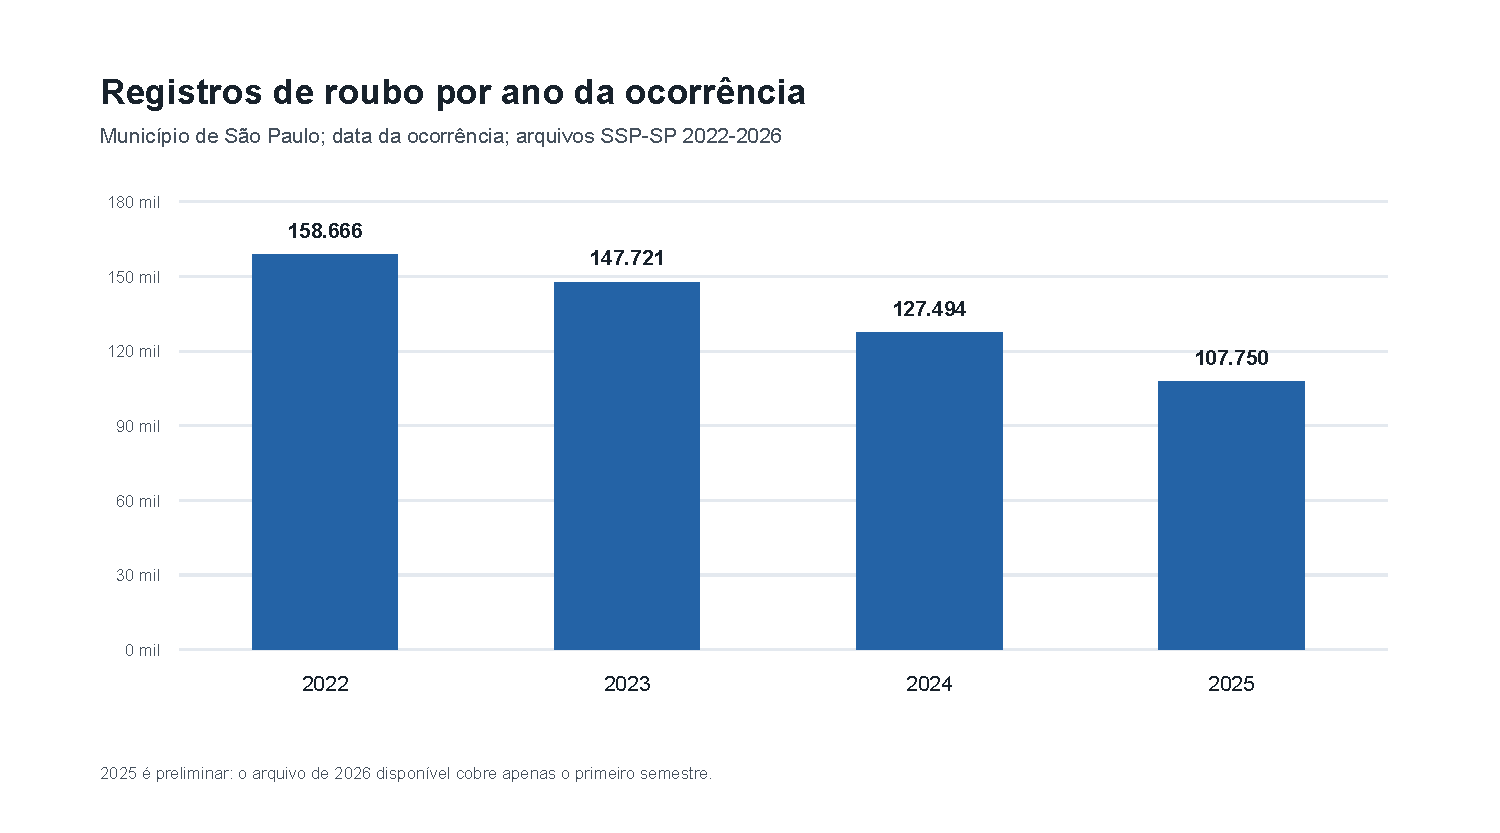
\includegraphics[width=0.83\linewidth]{roubos_por_ano.pdf}
  \caption{Registros classificados como roubo no município de São Paulo, por ano da ocorrência. Fonte: SSP-SP; elaboração própria.}
  \label{fig:ano}
\end{figure}

Em 2025, os arquivos disponíveis contêm 107.750 registros com data de ocorrência naquele ano, média aproximada de 295 por dia. A Figura~\ref{fig:semana} divide a contagem de cada dia da semana pelo número de vezes em que esse dia ocorreu no ano. As sextas-feiras tiveram média de 335 registros, enquanto domingos e segundas-feiras ficaram próximos de 254. A diferença é descritiva e sugere testar o dia da semana como variável do modelo, sem demonstrar capacidade preditiva por si só.

\begin{figure}[htbp]
  \centering
  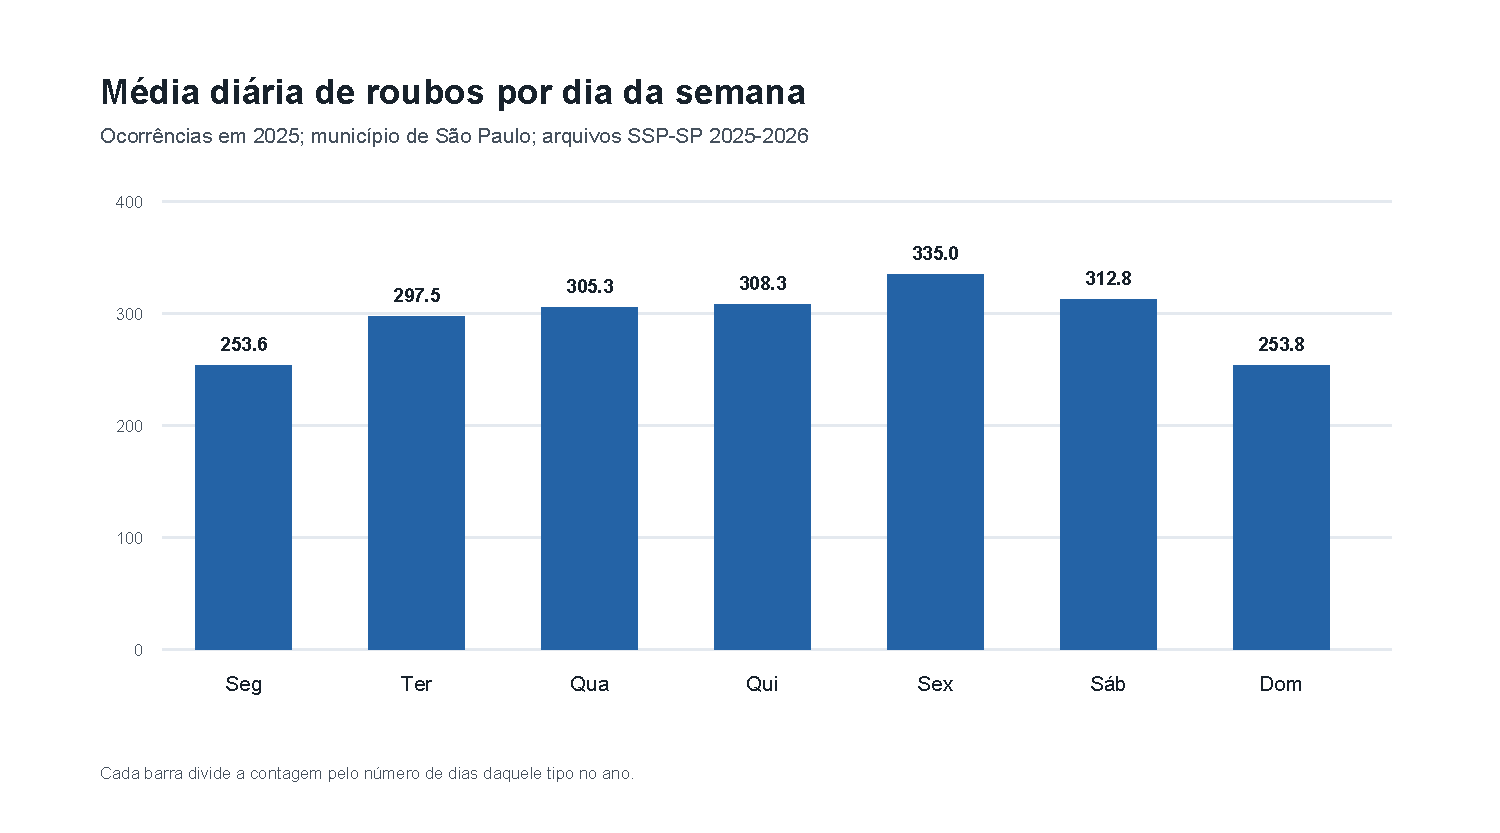
\includegraphics[width=0.83\linewidth]{roubos_por_dia_semana.pdf}
  \caption{Média diária de registros de roubo por dia da semana para fatos ocorridos em 2025. Fonte: SSP-SP; elaboração própria.}
  \label{fig:semana}
\end{figure}

A variação entre anos reforça a necessidade de avaliar os modelos em períodos posteriores aos de treinamento, pois os níveis de contagem observados no passado podem diferir daqueles encontrados no teste. Já as diferenças entre dias da semana orientam a inclusão de variáveis de calendário. Entretanto, esse padrão foi observado no total municipal e ainda precisa ser examinado por bairro: a média da cidade pode ocultar comportamentos locais distintos. Essas verificações ajudarão a escolher atributos e períodos de agregação adequados.

\subsection{Distribuição espacial e qualidade dos dados}

No arquivo de registros de 2025, foram encontrados 108.279 registros classificados como roubo e atribuídos ao município de São Paulo. A Figura~\ref{fig:bairros} mostra os dez rótulos de bairro com mais registros nesse arquivo. Capão Redondo aparece com 3.251, Campo Limpo com 2.460 e Pinheiros com 2.418. Esses valores são contagens absolutas, sem ajuste por população, área, circulação de pessoas ou subnotificação. Portanto, não representam taxas comparáveis de risco entre bairros.

\begin{figure}[htbp]
  \centering
  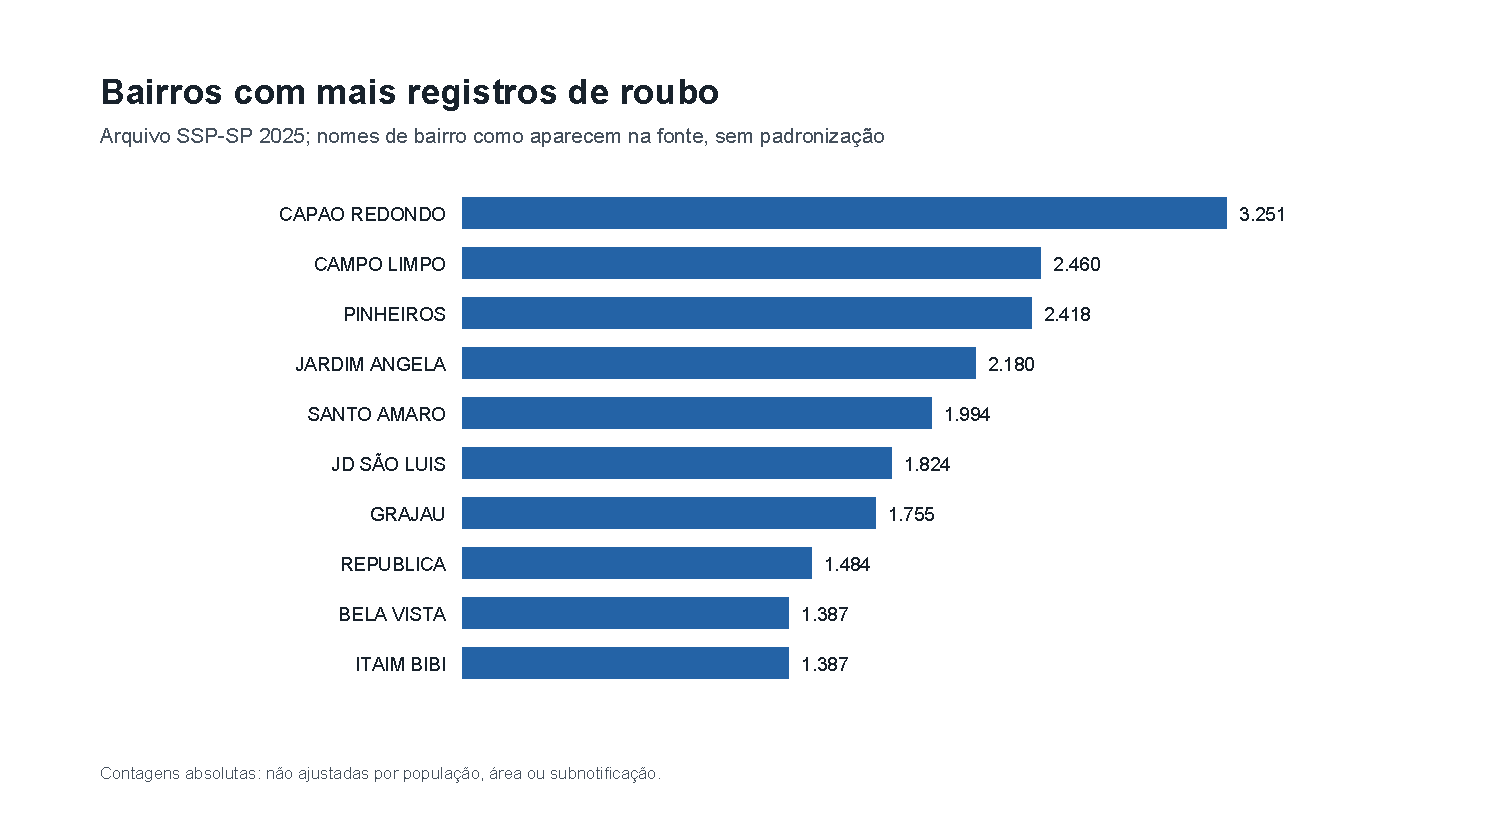
\includegraphics[width=0.83\linewidth]{roubos_bairros_2025.pdf}
  \caption{Bairros com mais registros de roubo no arquivo anual de 2025, sem padronização dos rótulos. Fonte: SSP-SP; elaboração própria.}
  \label{fig:bairros}
\end{figure}

No mesmo arquivo, 12.481 registros de roubo (11,5\%) têm coordenadas ausentes ou iguais a zero, e 416 (0,4\%) não têm bairro utilizável. Foram observados 1.895 rótulos distintos no campo de bairro, incluindo possíveis diferenças de grafia e abreviação. Um mapa construído apenas com coordenadas deixaria parte dos registros de fora; já a agregação por bairro exige revisar os rótulos antes de formar a série bairro--dia. Há também diferença entre o ano do registro e o da ocorrência: 106.888 dos 108.279 registros de roubo do arquivo de 2025 se referem a fatos ocorridos em 2025, enquanto outros registros têm datas anteriores. Por outro lado, o arquivo disponível de 2026 inclui 862 registros de fatos ocorridos em 2025.

Os rótulos distintos não correspondem necessariamente a bairros distintos. Variações de grafia podem dividir os registros de uma mesma área entre categorias, alterando tanto suas contagens quanto sua posição no gráfico. A padronização deverá reunir apenas equivalências verificadas, evitando juntar localidades diferentes. Para o mapa, também será necessário informar a proporção de registros efetivamente representados e verificar se a ausência de coordenadas varia entre áreas ou períodos, já que sua distribuição ainda não foi examinada.

\section{Discussão e Conclusão}

A análise exploratória confirmou que os microdados permitem estudar a contagem de registros de roubo ao longo dos dias e que há variação temporal e espacial relevante para a formulação de uma tarefa preditiva. A unidade bairro--dia continua sendo uma hipótese de trabalho, condicionada à padronização dos nomes de bairro e à verificação da frequência de dias com contagem zero. Também é necessário conferir a unicidade dos boletins antes de interpretar cada linha como um fato independente.

A integração de indicadores socioeconômicos, ainda não realizada, está alinhada ao objetivo de combinar informações de segurança com características das áreas analisadas. Esses indicadores poderão acrescentar contexto às diferenças de contagem, mas sua contribuição preditiva precisará ser avaliada. Antes do treinamento, será necessário compatibilizar as unidades geográficas e verificar a cobertura dos dados integrados. Posteriormente, comparar versões dos modelos com e sem esses atributos, sob a mesma divisão temporal, permitirá examinar se sua inclusão reduz os erros de previsão.

As contagens representam crimes registrados, não todos os crimes que ocorreram. Ausência de coordenadas, possíveis atrasos de registro e diferenças de cobertura entre regiões limitam interpretações de mapas e comparações entre bairros. Nenhum modelo foi treinado nesta etapa; assim, não há medida de acurácia nem mapa de previsão. Os próximos passos são consolidar as contagens por área e período, compatibilizar os indicadores socioeconômicos, definir uma referência simples, treinar os modelos com divisão temporal e comparar seus erros em períodos posteriores aos usados no treinamento.

\renewcommand{\refname}{Referências}
\begin{thebibliography}{9}

\bibitem{ssp} SSP-SP -- Secretaria da Segurança Pública do Estado de São Paulo. \textit{Estatísticas da Criminalidade -- Consultas}. Disponível em: \url{https://www.ssp.sp.gov.br/estatistica/consultas}. Acesso em: 27 set. 2026.

\bibitem{ibge} IBGE -- Instituto Brasileiro de Geografia e Estatística. \textit{Censo Demográfico 2022}. Disponível em: \url{https://www.ibge.gov.br/estatisticas/sociais/populacao/22827-censo-demografico-2022.html}. Acesso em: 27 set. 2026.

\bibitem{ribeiro2022} RIBEIRO, J. S.; MENESES, L.; COSTA, D. C. L.; MIRANDA, W. D.; ALVES, R. \textit{Prediction of Homicides in Urban Centers: A Machine Learning Approach}. In: Intelligent Systems and Applications, 2022, p. 344--361. DOI: \url{https://doi.org/10.1007/978-3-030-82199-9_22}.

\bibitem{crimanalyzer} GARCÍA-ZANABRIA, G. et al. \textit{CrimAnalyzer: Understanding Crime Patterns in São Paulo}. IEEE Transactions on Visualization and Computer Graphics, v. 27, n. 4, p. 2313--2328, 2021. DOI: \url{https://doi.org/10.1109/TVCG.2019.2947515}.

\bibitem{hassan2024} HASSAN, W. et al. \textit{Modeling and Predicting Crimes in the City of São Paulo Using Graph Neural Networks}. In: BRACIS, 2024, p. 372--386. Disponível em: \url{https://sol.sbc.org.br/index.php/bracis/article/view/33639}.

\end{thebibliography}

\end{document}
